\documentclass[aspectratio=169,11pt]{beamer}

\usetheme{auriga}
\usecolortheme{auriga}

\usepackage{booktabs}
\usepackage{tikz}
\usetikzlibrary{positioning,shapes.geometric,arrows.meta,calc}
\usepackage{graphicx}
\graphicspath{{../report/figures/}}

% Accent + flag colours
\definecolor{accent}{RGB}{0,113,150}
\definecolor{ethgreen}{RGB}{0,141,98}
\definecolor{ethyellow}{RGB}{252,210,0}
\definecolor{ethred}{RGB}{218,18,26}
\definecolor{ethblue}{RGB}{0,71,171}
\definecolor{nggreen}{RGB}{0,135,81}
\definecolor{kered}{RGB}{187,0,0}
\definecolor{kegreen}{RGB}{0,98,51}
\setbeamercolor{frametitle}{fg=accent}

\title{Confidently Wrong}
\author{Calibration Risks and Safe Abstention in LLMs for African Languages}

% Reusable three-flags graphic (Ethiopia, Nigeria, Kenya)
\newcommand{\teamflags}[1][1]{%
\begin{tikzpicture}[scale=#1, every node/.style={scale=#1}]
  % ---- Ethiopia ----
  \begin{scope}[shift={(0,0)}]
    \fill[ethgreen]  (0,1.0667) rectangle (2.4,1.6);
    \fill[ethyellow] (0,0.5333) rectangle (2.4,1.0667);
    \fill[ethred]    (0,0)      rectangle (2.4,0.5333);
    \fill[ethblue] (1.2,0.8) circle (0.46);
    \node[star, star points=5, star point ratio=2.3, fill=ethyellow,
          draw=ethyellow, minimum size=7.5mm, inner sep=0pt] at (1.2,0.8) {};
    \draw[black,line width=0.4pt] (0,0) rectangle (2.4,1.6);
    \node[font=\scriptsize] at (1.2,-0.35) {Ethiopia};
  \end{scope}
  % ---- Nigeria ----
  \begin{scope}[shift={(3.6,0)}]
    \fill[white]   (0,0)   rectangle (2.4,1.6);
    \fill[nggreen] (0,0)   rectangle (0.8,1.6);
    \fill[nggreen] (1.6,0) rectangle (2.4,1.6);
    \draw[black,line width=0.4pt] (0,0) rectangle (2.4,1.6);
    \node[font=\scriptsize] at (1.2,-0.35) {Nigeria};
  \end{scope}
  % ---- Kenya ----
  \begin{scope}[shift={(7.2,0)}]
    \fill[black]   (0,1.12) rectangle (2.4,1.6);
    \fill[white]   (0,1.04) rectangle (2.4,1.12);
    \fill[kered]   (0,0.56) rectangle (2.4,1.04);
    \fill[white]   (0,0.48) rectangle (2.4,0.56);
    \fill[kegreen] (0,0)    rectangle (2.4,0.48);
    \draw[white,line width=1.3pt] (0.98,0.25) -- (1.42,1.35);
    \draw[white,line width=1.3pt] (1.42,0.25) -- (0.98,1.35);
    \fill[kered] (1.2,0.8) ellipse (0.2 and 0.42);
    \draw[white,line width=0.9pt] (1.2,0.8) ellipse (0.2 and 0.42);
    \fill[white] (1.08,0.77) rectangle (1.32,0.83);
    \draw[black,line width=0.4pt] (0,0) rectangle (2.4,1.6);
    \node[font=\scriptsize] at (1.2,-0.35) {Kenya};
  \end{scope}
\end{tikzpicture}}

\begin{document}

% ============================== 1. Title ==============================
\begin{frame}[plain]
  \centering
  \vskip1ex
  \teamflags[1.0]\par
  \vskip4ex
  {\LARGE\bfseries Confidently Wrong\par}
  \vskip1.5ex
  {\large Calibration Risks and Safe Abstention\\ in LLMs for African Languages\par}
  \vskip4ex
  {\footnotesize Similoluwa Okunowo \quad Eliud Koto \quad Dagmawi Misker\par}
  \vskip1ex
  {\scriptsize African Institute for Mathematical Sciences (AIMS), South Africa \quad$\cdot$\quad With Apart Research\par}
  \vskip1ex
  {\scriptsize\itshape A team from Ethiopia, Nigeria, and Kenya \quad$\cdot$\quad Global South AI Safety Hackathon, June 2026\par}
\end{frame}

% ============================== 2. Problem ==============================
\begin{frame}{The problem}
  \begin{itemize}
    \item LLMs are increasingly used in African languages, but their reliability there is largely \textbf{unmeasured}.
    \item The failure we study is being \textbf{confidently wrong}: a wrong answer delivered with high confidence.
    \item A miscalibrated model, whose confidence does not track its accuracy, cannot know when to \textbf{abstain}.
  \end{itemize}
\end{frame}

% ============================== 3. Significance ==============================
\begin{frame}{Why it matters for African AI safety}
  \begin{itemize}
    \item These models answer \textbf{high-stakes} questions: health, legal, educational, civic.
    \item Users often \textbf{cannot verify} an answer in their own language.
    \item If calibration holds in English but breaks in African languages, the populations \textbf{least served} are the most exposed to confident misinformation.
  \end{itemize}
\end{frame}

% ============================== 4. Methods ==============================
\begin{frame}{Methods}
  \begin{itemize}
    \item \textbf{Four open models:} Qwen3-4B-Instruct, Gemma-4-12B, Aya-Expanse-8B, AfroLlama-V1.
    \item \textbf{Two benchmarks:} Uhura-TruthfulQA (truthfulness) and AfriMMLU (knowledge).
    \item \textbf{Scoring:} length-normalised answer-text log-probability (robust to instruction-tuned models).
    \item \textbf{Metrics \& interventions:} ECE, overconfidence, AUROC, AUARC; temperature scaling, abstention, few-shot.
  \end{itemize}
\end{frame}

% ============================== 5. Result: the gap ==============================
\begin{frame}{Result: calibration degrades in African languages}
  \begin{columns}[c]
    \begin{column}{0.52\textwidth}
      \begin{itemize}
        \item ECE and overconfidence are markedly higher in African languages, across models and tasks.
        \item Models are most overconfident exactly where they are least accurate.
      \end{itemize}
    \end{column}
    \begin{column}{0.46\textwidth}
      \footnotesize
      \centering
      \begin{tabular}{lcc}
        \toprule
        \textbf{Model (Uhura)} & \textbf{ECE en} & \textbf{ECE afr}\\
        \midrule
        Qwen3-4B      & 0.07 & 0.17\\
        Gemma-4-12B   & 0.21 & 0.26\\
        Aya-Expanse-8B& 0.08 & 0.20\\
        \bottomrule
      \end{tabular}
    \end{column}
  \end{columns}
\end{frame}

% ============================== 6. Result: figure ==============================
\begin{frame}{Result: calibration error by language}
  \centering
  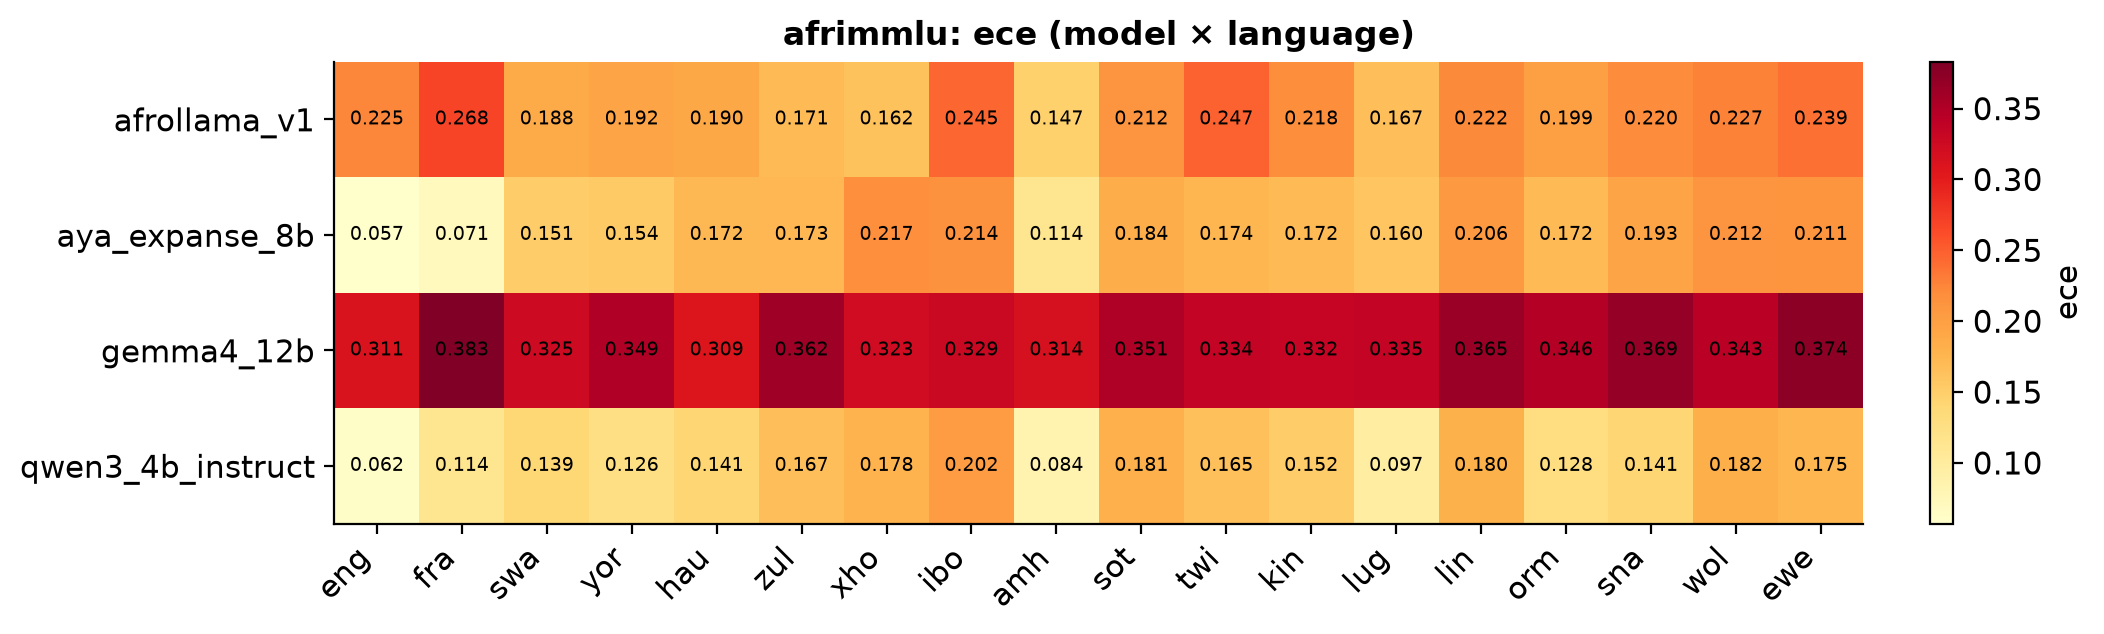
\includegraphics[width=0.92\textwidth,height=0.78\textheight,keepaspectratio]{afrimmlu_ece_heatmap.png}\\[0.5ex]
  {\footnotesize ECE is low in English and French and rises across African languages.}
\end{frame}

% ============================== 7. Result: mitigations ==============================
\begin{frame}{Result: mitigations are unequal}
  \begin{itemize}
    \item \textbf{Temperature scaling} is the clear winner: per-language recalibration cuts ECE to $\approx 0.03$, with no retraining.
    \item \textbf{Abstention} helps less: the uncertainty signal is weak (AUROC $\approx 0.55$).
    \item \textbf{Few-shot} prompting helps three models but \textbf{backfires on Gemma-4-12B}.
    \item \textbf{Bigger is not safer:} the 12B model is the worst calibrated.
  \end{itemize}
\end{frame}

% ============================== 8. Deployment framework ==============================
\begin{frame}{Deployment framework}
  \centering
  \resizebox{!}{0.66\textheight}{%
  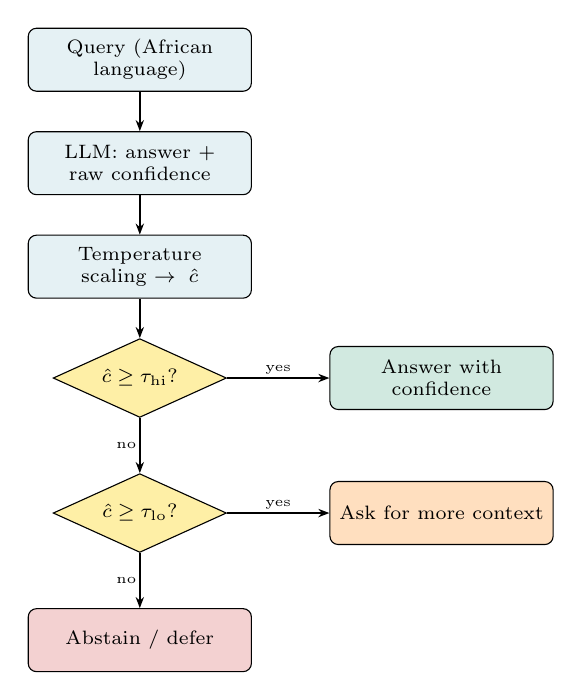
\begin{tikzpicture}[
    node distance=5mm and 13mm,
    box/.style={rectangle, rounded corners=3pt, draw, align=center, font=\scriptsize,
                text width=26mm, minimum height=8mm},
    proc/.style={box, fill=accent!10},
    dec/.style={diamond, draw, fill=ethyellow!35, aspect=2.2, align=center,
                font=\scriptsize, inner sep=1pt, text width=15mm},
    good/.style={box, fill=nggreen!18}, warn/.style={box, fill=orange!25}, bad/.style={box, fill=kered!18},
    arr/.style={-{Stealth[length=4pt]}, semithick},
    lbl/.style={font=\tiny, inner sep=1pt}]
    \node[proc] (q) {Query (African language)};
    \node[proc, below=of q] (m) {LLM: answer $+$ raw confidence};
    \node[proc, below=of m] (ts) {Temperature scaling $\rightarrow \hat{c}$};
    \node[dec, below=of ts] (d1) {$\hat{c}\!\ge\!\tau_{\mathrm{hi}}$?};
    \node[dec, below=7mm of d1] (d2) {$\hat{c}\!\ge\!\tau_{\mathrm{lo}}$?};
    \node[bad, below=7mm of d2] (ab) {Abstain / defer};
    \node[good, right=of d1] (ans) {Answer with confidence};
    \node[warn, right=of d2] (ctx) {Ask for more context};
    \draw[arr] (q)--(m); \draw[arr] (m)--(ts); \draw[arr] (ts)--(d1);
    \draw[arr] (d1)--(d2) node[lbl,midway,left]{no};
    \draw[arr] (d2)--(ab) node[lbl,midway,left]{no};
    \draw[arr] (d1)--(ans) node[lbl,midway,above]{yes};
    \draw[arr] (d2)--(ctx) node[lbl,midway,above]{yes};
  \end{tikzpicture}}\\[1ex]
  {\footnotesize Recalibrate first, then route on calibrated confidence; thresholds $\tau$ set per language.}
\end{frame}

% ============================== 9. Limitations & Future work ==============================
\begin{frame}{Limitations \& future work}
  \begin{itemize}
    \item Accuracies sit near chance on these hard tasks; ECE gaps may partly reflect translation quality.
    \item Abstention is bounded by a weak uncertainty signal, so recalibration is the more reliable lever.
    \item \textbf{Next:} reasoning and closed models; in-context calibration at scale; native-speaker audits and human-grounded abstention.
  \end{itemize}
\end{frame}

% ============================== 10. Conclusion ==============================
\begin{frame}{Takeaways}
  \begin{itemize}
    \item Open LLMs are \textbf{confidently wrong} in African languages: less accurate, more overconfident.
    \item Cheap, post-hoc \textbf{temperature scaling} is a deployable safety lever today.
    \item Pair recalibration with \textbf{thresholded abstention} for safer real-world use.
  \end{itemize}
\end{frame}

% ============================== 11. Thank you ==============================
\begin{frame}[plain]
  \centering
  \vskip2ex
  \teamflags[0.9]\par
  \vskip5ex
  {\LARGE\bfseries Thank you\par}
  \vskip2ex
  {\scriptsize\ttfamily github.com/rexsimiloluwah/aims-team-apart-ai-safety-hackathon\par}
\end{frame}

\end{document}
